% !TeX program = xelatex
% MetaCircle arXiv source. Build with: latexmk -xelatex main.tex
\documentclass[11pt]{article}
\usepackage[round,authoryear]{natbib}
\PassOptionsToPackage{no-math}{fontspec}
\usepackage{metacircle}
\usepackage{float}
\usepackage{array}
\usepackage{multirow}

\renewcommand{\topfraction}{0.95}
\renewcommand{\bottomfraction}{0.5}
\renewcommand{\textfraction}{0.05}
\renewcommand{\floatpagefraction}{0.8}
\graphicspath{{figures/}}

\newcommand{\KL}{\operatorname{KL}}
\newcommand{\Var}{\operatorname{Var}}
\newcommand{\E}{\mathbb{E}}
\newcommand{\RMS}{\operatorname{RMS}}
\newcommand{\q}{q}
\newcommand{\p}{p}
\newcommand{\pt}{p_t}
\newcommand{\pzero}{p_0}

\title{Explanation of RGI:\\Shared Batch Difficulty and Setting-Dependent Gaps}
\author{
  Shaoyang Guo$^{*}$ and Ziming Liu$^{\dagger}$\\
  \small $^*$Core author \quad $^\dagger$Corresponding author
}
\date{}
\paperdate{October 8, 2026}
\papertype{Meta Circle Research}
\projecturl{https://guoshaoyang-pku.github.io/RGI-explained/}

\begin{document}
\maketitle

\begin{metaabstract}
We study what is shared, and what is optimizer-dependent, in teacher-forced language-model loss.  The recent Relative Generalization Invariance (RGI) result reports that token-wise loss differences can remain highly similar across training choices, but it does not identify the finite-update terms responsible for a Transformer trajectory.  We decompose an arriving-batch loss into a frozen-data difficulty and a local response.  For an update from \(\theta_0\) to \(\theta_t\), the response has an exact linear-work term \(A=\nabla_\theta\ell(\theta_0)^\top(\theta_t-\theta_0)\), a nonnegative logit-space curvature term \(Q=\operatorname{KL}(p_0\Vert p_t)\), and a representation residual.  Its second-order logit approximation is \(A+Q_2\), with \(Q_2=\tfrac12\operatorname{Var}_{p_0}(\Delta z)\).

Across three permutations of a fixed FineWeb pool and SGD or Adam continuation of Pythia-70M, a common step-32,000 reference explains 96.657--97.582\% of arriving-loss variance; each algorithm's frozen start explains 99.940--99.997\% in the registered near and far windows.  On the residual slow signal \(L-D\), observed-displacement \(A+Q_2\) has 4.97--9.73\% relative RMS error for SGD and 1.19--2.82\% for Adam, with at least 96.87\% variance explained.  Signed covariance shows negative linear work and positive curvature cancel, and both terms change with the optimizer.  A single scalar probe does not close the batch-specific response, and the optimizer difference fails the 10\% response gate.  A fixed-teacher continuation closes the same local decomposition, but its cross-prefix optimizer gap still fails a strict constant-offset test.  We therefore obtain a quantitative local finite-displacement mechanism and a clear boundary: the evidence does not establish a universal strong-RGI mechanism for natural language models.

\keywords{language model training, teacher forcing, optimization dynamics, relative generalization invariance, cross-entropy}
\end{metaabstract}

\section{Introduction}

The loss of a language model mixes two sources of variation that are usually reported together.  A batch can be intrinsically difficult under a fixed predictor, while the predictor can also move during training.  The first source changes when the next batch changes; the second accumulates through the optimizer and the model's local geometry.  A useful explanation of training loss should identify these terms on the same teacher-forced targets and should say which term dominates at the scale being measured.

Zhang et al.~\citep{zhang2026relativegeneralizationinvariancellm} introduced Relative Generalization Invariance (RGI): the validation-loss difference between two models is approximately preserved across tokens.  Their experiments show strong empirical similarity across optimizers and moderate architectural changes, while their quadratic example gives a sufficient stylized construction.  The result leaves open a more local question: when a real Transformer receives one arriving batch, which terms create the common fast variation, and which terms create the slower optimizer-dependent response?  This distinction matters because high correlation of two loss curves does not imply a constant token-wise gap.

We test the following concrete version of the question.  Let \(D(B)\) be the teacher-forced cross-entropy of a fixed start model on batch \(B\), let \(L_t(B)\) be the same score after an observed continuation, and write \(M_t(B)=L_t(B)-D(B)\).  We ask whether \(D\) explains the large batch-to-batch variation, and whether \(M\) is explained by a frozen gradient acting on the observed parameter displacement plus softmax curvature.  We do not fit a slope or intercept on the evaluation window, and we do not treat an identity using the final logits as a forecast of an unknown future update.

Our contributions are:
\begin{itemize}
  \item We give a teacher-forced, batch-level decomposition that separates frozen difficulty from finite local response and measures each term directly.
  \item In a registered Pythia-70M continuation, a common frozen reference explains 96.657--97.582\% of raw arriving-loss variance, while the algorithm-specific frozen starts explain at least 99.940\% in the far window.
  \item On the slow signal itself, \(A+Q_2\) closes all six natural near, far, and full windows at the registered 10\% RMS and 90\% variance thresholds.  The signed terms show that linear learning gain and positive curvature cost both matter.
  \item We document the boundary of this explanation: a scalar global probe is insufficient, the optimizer-difference response fails the 10\% gate, and a known-teacher population test does not yield a constant token-wise optimizer offset.
\end{itemize}

The claims are deliberately local.  We study finite Pythia-70M continuations with reset optimizer state, not a reproduction of the original paper's 124M and 0.7B pretraining runs.  The main conclusion is a measured response mechanism for these trajectories, together with a substantive obstruction to promoting it to a universal explanation of strong RGI.

\section{Relation to RGI and scope of the claim}

RGI compares a pair of models on the same teacher-forced target and asks whether their loss difference is approximately independent of the token.  We retain that paired evaluation, but separate two notions that are easy to conflate.  A weak statement is that two loss vectors have high correlation or a small relative-difference statistic.  A strong statement is that
\begin{equation}
  \ell_A(x,y)-\ell_B(x,y) \approx c
  \quad\text{for every evaluated prefix--target pair,}
  \label{eq:strong-rgi}
\end{equation}
with a residual small relative to \(|c|\).  The latter is the constant-offset mechanism that would make the optimizer choice nearly irrelevant to token ranking.

Our experiment is designed to locate terms before testing Eq.~\eqref{eq:strong-rgi}.  On a natural target, an arbitrary checkpoint reference \(q\) is not the unknown conditional data distribution.  Therefore a reference KL is a measurable comparison to \(q\), not a natural Bayes excess risk.  For a fixed teacher distribution we can remove this ambiguity, but that changes the task to a known-teacher continuation.  We report the two settings separately.

The prior quadratic construction is a sufficient example in a different model class.  It does not by itself identify the representation term or optimizer response of a Transformer.  Our evidence likewise does not claim that natural LLMs satisfy the sufficient conditions of that construction.  Instead, it tests whether the more concrete finite-displacement terms below account for the observed slow response and then checks whether the remaining paired gap is actually constant.

\paragraph{Relation to normalized gradient flow.}
Lee and Lee~\citep{lee2026journeyedgestability} report nearly coincident low-learning-rate loss and sharpness traces for fixed linear gradient filters on CIFAR-10, after normalizing the effective step \(h=\eta\mathcal{Q}(1)\) and progress \(\tau=th\) by the filter's dc gain.  Their local modified-flow expansion, for a smooth objective and stable filter with slowly varying gradients through its memory, is
\begin{equation}
  \frac{d\theta}{d\tau}=-g-h\alpha_{\mathcal{Q}}Hg+O(h^2),
  \qquad \alpha_{\mathcal{Q}}=\frac12-\frac{\mathcal{Q}'(1)}{\mathcal{Q}(1)}.
  \label{eq:filterflow}
\end{equation}
The leading flow is shared while the filter shape changes the next correction.  Their consecutive-gradient cosine compares adjacent iterations inside a run, not parameters across optimizers.  Preconditioning is outside that study's scope; Adam is consequently an additional empirical intervention here, rather than an instance of its scalar dc normalization.

Shared leading flow does not imply a nonzero constant token-wise loss offset.  Even nearby points on one flow have a first-order loss difference proportional to \(g_i^\top g_{\mathrm{train}}\), which depends on the scored token \(i\).  The proposed connection is therefore precise: low-step alignment may constrain the response differences in Eq.~\eqref{eq:paired}, while their centered sample structure still requires direct measurement.  Our rate labels describe a controlled rate contrast; without measured stability geometry they do not identify an edge-of-stability regime.

\section{A finite-update decomposition}

Consider one prefix--target pair \((x,y)\), with logits \(z_0(x)\) at the frozen start \(\theta_0\), probabilities \(p_0=\operatorname{softmax}(z_0)\), and logits \(z_t\) after the observed continuation.  Write \(\Delta z=z_t-z_0\), \(p_t=\operatorname{softmax}(z_t)\), and \(e_y\) for the one-hot target.  For a batch, all quantities below are averaged over the same target positions.

The frozen difficulty is
\begin{equation}
  D(B)=\operatorname{mean}_{(x,y)\in B}\left[-\log p_0(y\mid x)\right].
  \label{eq:difficulty}
\end{equation}
The exact change in cross-entropy has a useful logit-space identity,
\begin{align}
  L_t(B)-D(B)&=W(B)+Q(B),\\
  W(B)&=\operatorname{mean}\left[(p_0-e_y)^\top\Delta z\right],\\
  Q(B)&=\operatorname{mean}\left[\KL(p_0\Vert p_t)\right]\geq 0.
  \label{eq:exact}
\end{align}
The equality follows from the log-partition identity and is used as an arithmetic check.  It is not a forecast because it uses the observed final logits.

To connect the loss change to parameter motion, recompute the batch gradient at \(\theta_0\) and define
\begin{equation}
  A(B)=\nabla_\theta\ell_{\theta_0}(B)^\top(\theta_t-\theta_0),
  \qquad R(B)=W(B)-A(B).
  \label{eq:work}
\end{equation}
The exact change can then be written \(L_t-D=A+R+Q\).  The residual \(R\) includes the nonlinearity of the parameter-to-logit map along the observed displacement, as well as any replay or numerical error; we do not identify it with a single unmeasured Hessian term.

The second-order logit approximation to the convex log-partition term is
\begin{equation}
  Q_2(B)=\frac12\operatorname{mean}_{(x,y)\in B}\left[\operatorname{Var}_{v\sim p_0(\cdot\mid x)}\left(\Delta z_v(x)\right)\right].
  \label{eq:q2}
\end{equation}
Our primary local closure is therefore \(L_t-D\approx A+Q_2\).  Both \(A\) and \(Q_2\) use the displacement that actually occurred: \(A\) uses \(\theta_t-\theta_0\), and \(Q_2\) uses \(\Delta z\).  The test explains a realized finite response; it does not predict a future response from a frozen gradient alone.

For a fixed teacher distribution \(q(\cdot\mid x)\), the same algebra replaces \(e_y\) by \(q\).  With \(p_t=\operatorname{softmax}(z_q+v)\), the teacher-forced hard-target loss decomposes as
\begin{equation}
  \ell=S+C+E,\qquad S=-\log q_y,\quad C=(q-e_y)^\top v,\quad E=\KL(q\Vert p_t).
  \label{eq:teacher}
\end{equation}
Under a target drawn from \(q\), \(\mathbb{E}_q[C\mid x]=0\), and the population cross-entropy is \(H(q)+E\).  We use this controlled population objective to separate label sampling from the natural-text case, where the unknown conditional distribution is not observed.

\section{Experimental protocol}

\paragraph{Natural continuation.}
We use the public Pythia-70M architecture~\citep{biderman2023pythiasuiteanalyzinglarge} and official step-32,000 checkpoint as the shared reference and continue the model locally.  The model has 70,426,624 trainable parameters and the verified Pythia tokenizer has vocabulary size 50,304.  The new data pool contains 4,672 length-qualified FineWeb sample-10BT documents~\citep{penedo2024finewebdatasetsdecantingweb} from revision \texttt{9bb295dd...}, with source rows beginning at 65,536.  We select one random 256-token span per document, exclude registered prior IDs, text hashes, and exact spans, and split 4,096/64/512 documents into training, calibration, and evaluation pools.  Selection used no model score.  The data source is not claimed to be absent from Pythia pretraining or to be domain extrapolation.

Three fixed permutations of the same pool are run for 512 updates with batch size 8 and context length 256.  The continuation starts from the corresponding completed SGD or Adam trajectory and resets optimizer state.  SGD uses learning rate \(10^{-3}\); Adam~\citep{kingma2017adammethodstochasticoptimization} uses learning rate \(10^{-6}\), betas \((0.9,0.95)\), and \(\epsilon=10^{-8}\).  These are controlled local continuations, not the historical Pythia AdamW/Pile pretraining process.  The common frozen reference \(q\) is the official step-32,000 model; each algorithm also has its own frozen start \(p_0\).

\paragraph{Known teacher.}
The teacher is the official step-32,000 model.  From 33-token natural seeds, it samples 63 autoregressive tokens at temperature one using the full 50,304-token vocabulary.  The resulting 1,216 documents are split 1,024/64/128 for training, calibration, and evaluation.  A student starts from official step 16,000 and trains for 128 updates under either hard sampled targets or the full soft teacher distribution~\citep{hinton2015distillingknowledgeneuralnetwork}, with the same three permutations and two optimizers.  This is a synthetic known-teacher conditional task, not an estimate of the natural Bayes distribution.

\paragraph{Readouts and gates.}
For each arriving batch we record teacher-forced \(L_t\), frozen \(D\), \(A\), \(W\), \(Q\), \(Q_2\), and \(R\).  We predeclare near \(0{:}128\), far \(384{:}512\), and full \(0{:}512\) windows.  Relative RMS error and variance explained \(1-\operatorname{MSE}/\operatorname{Var}\) are reported separately.  The primary gates are 10\% relative RMS and 90\% variance explained.  We also report 64-step block means, high-pass residuals, and signed covariance shares \(\operatorname{Cov}(M,T)/\operatorname{Var}(M)\), which can be negative and sum to one.

The frozen-difficulty windows were registered before the fresh continuation.  The arrival-batch and logit-work analyses are retrospective diagnostics of completed trajectories.  Independent verifiers checked saved traces, hashes, identities, and fixtures; they did not independently recompute the full network gradients or the complete parameter trajectories.

\section{The four measured curves and their validity range}
\label{sec:common-results}

Table~\ref{tab:core} is the central result.  It separates the shared batch scale from each training setting's signed linear work, positive variance cost, and measured remainder.  The terminal local-scale protocol is shown first; the earlier failed rate protocols remain in Table~\ref{tab:rate-validity} and the supplementary four-term figures.  Each range spans three paired permutations of one reused data pool, not a confidence interval or independent dataset replications.

\begin{table}[t]
\centering
\caption{Core four-term table for common step-143,000 starts and 512 arrivals.  SGD/HB and head-only use effective rate $3\times10^{-8}$; Adam's calibrated rate is $3.02668\times10^{-9}$.  HB denotes normalized Heavy Ball.  Scaled nats are explicit in each row.  The statistics deliberately differ: batch standard deviation for $D$, signed means for $A,Q_2$, and RMS for $\varepsilon$.  Six-setting tables, including the tenfold larger rate, are retained in the supplement.}
\label{tab:core}
\setlength{\tabcolsep}{3.5pt}
\small
\begin{tabular}{lrrrr}
\toprule
Term and statistic & SGD & HB & Adam & Head only \\
\midrule
$D$: batch std. (nats) & $0.18530\;\text{to}\;0.18634$ & $0.18530\;\text{to}\;0.18634$ & $0.18530\;\text{to}\;0.18634$ & $0.18530\;\text{to}\;0.18634$ \\
$A$: mean ($10^{-4}$ nats) & $-1.78\;\text{to}\;-1.76$ & $-1.76\;\text{to}\;-1.75$ & $-6.60\;\text{to}\;-6.56$ & $-0.95\;\text{to}\;-0.94$ \\
$Q_2$: mean ($10^{-5}$ nats) & $1.08\;\text{to}\;1.26$ & $1.07\;\text{to}\;1.26$ & $1.12\;\text{to}\;1.13$ & $0.14\;\text{to}\;0.15$ \\
$\varepsilon$: RMS ($10^{-5}$ nats) & $2.42\;\text{to}\;3.49$ & $2.43\;\text{to}\;3.53$ & $0.26\;\text{to}\;0.29$ & $(2.76\;\text{to}\;2.86)\!\times\!10^{-4}$ \\
\bottomrule
\end{tabular}

\end{table}

\begin{figure}[t]
\centering
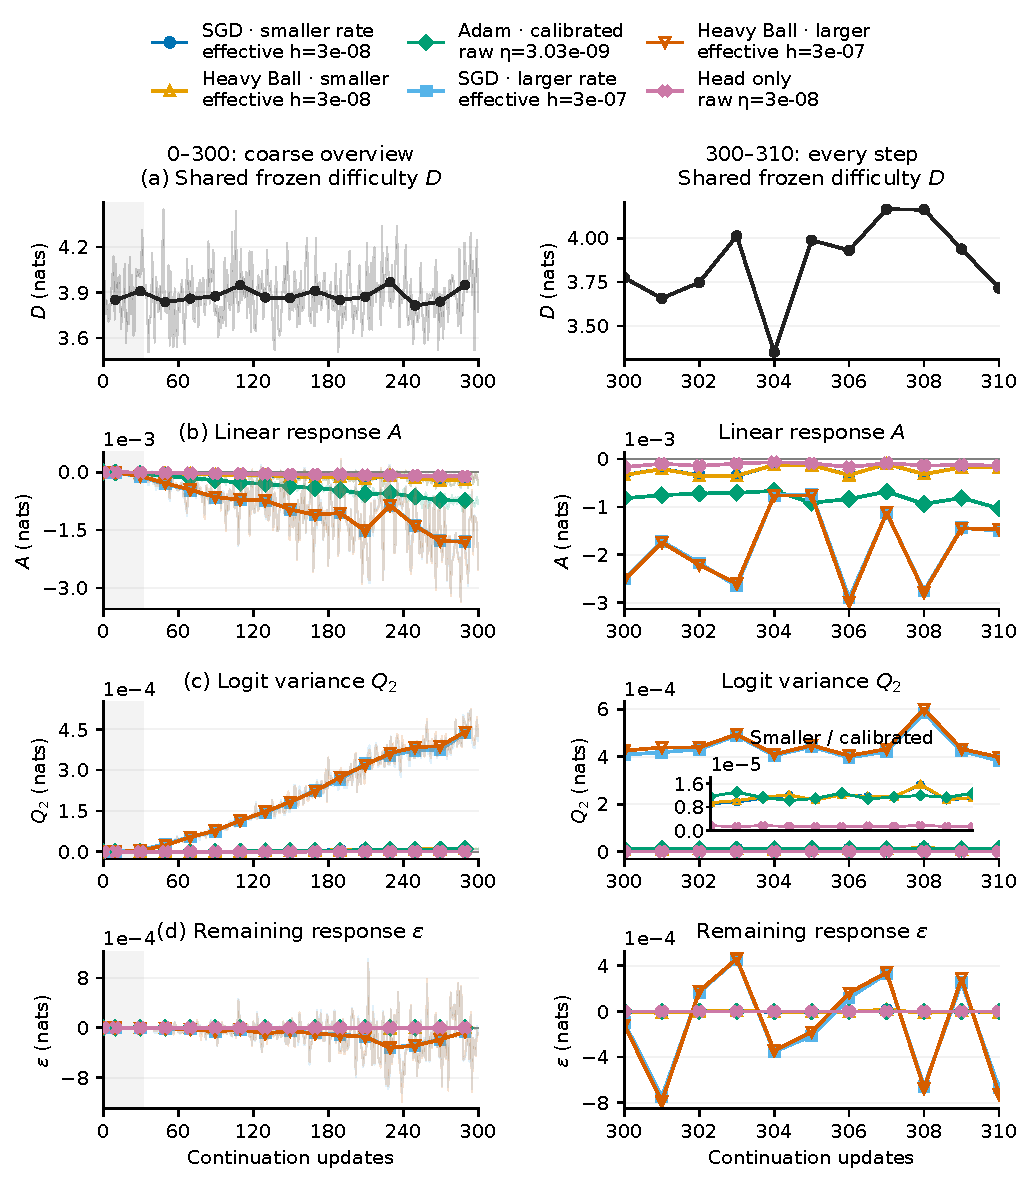
\includegraphics[width=\linewidth]{common-local-arriving.pdf}
\caption{Four terms on the common arriving-batch stream, with permutation zero fixed before results.  The shared frozen $D$ is drawn once.  Thin raw traces and prespecified 64-step block means are retained; all panels use nats with independent vertical scales.  Shading marks the 32-update warmup.  $A,Q_2,\varepsilon$ begin at zero; $D$ varies because the arriving batch changes.  Full six-setting curves are shown, including the tenfold larger rates.}
\label{fig:four-arrival}
\end{figure}

\paragraph{Shared difficulty dominates raw loss at the local scale.}
For the terminal protocol, every setting's frozen prediction fraction exceeds 99.9926\%.  The shared batch standard deviation of $D$ is 0.18530--0.18634 nats, while mean work and variance are orders of magnitude smaller.  This establishes dominance of frozen batch difficulty in these raw arriving losses.  It does not establish stochastic independence, a natural Bayes entropy, or a common optimizer-response coefficient.

\paragraph{Response closure is conditional, even at small rates.}
Adam passes the full-window response gate at 0.3387--0.3748\% relative RMS.  The affine head-only control passes at 0.002410--0.002470\%.  SGD and normalized HB narrowly fail at 10.51--14.96\% and 10.56--15.21\%, respectively.  Their near windows pass (SGD 1.89--7.13\%, HB 1.82--7.12\%), but far windows fail (SGD 12.14--18.44\%, HB 12.15--18.77\%).  Thus small update size is not sufficient for a uniformly small remainder across an accumulated 512-update displacement.  These failures are retained rather than treating the raw loss's near-perfect agreement as a passed mechanism test.

In all terminal settings, $A$ has a negative mean and $Q_2$ a positive mean.  On the full raw response, the signed covariance shares for low SGD are 1.007--1.033 for $A$, $-0.0457$ to $-0.0347$ for $Q_2$, and 0.0131--0.0322 for $\varepsilon$.  For Adam they are 1.020--1.021, $-0.0235$ to $-0.0230$, and 0.00263--0.00279.  Linear work dominates response variation and curvature offsets some of it.  These descriptive signed shares account for cancellation and do not identify independent causal percentages.

\begin{figure}[t]
\centering
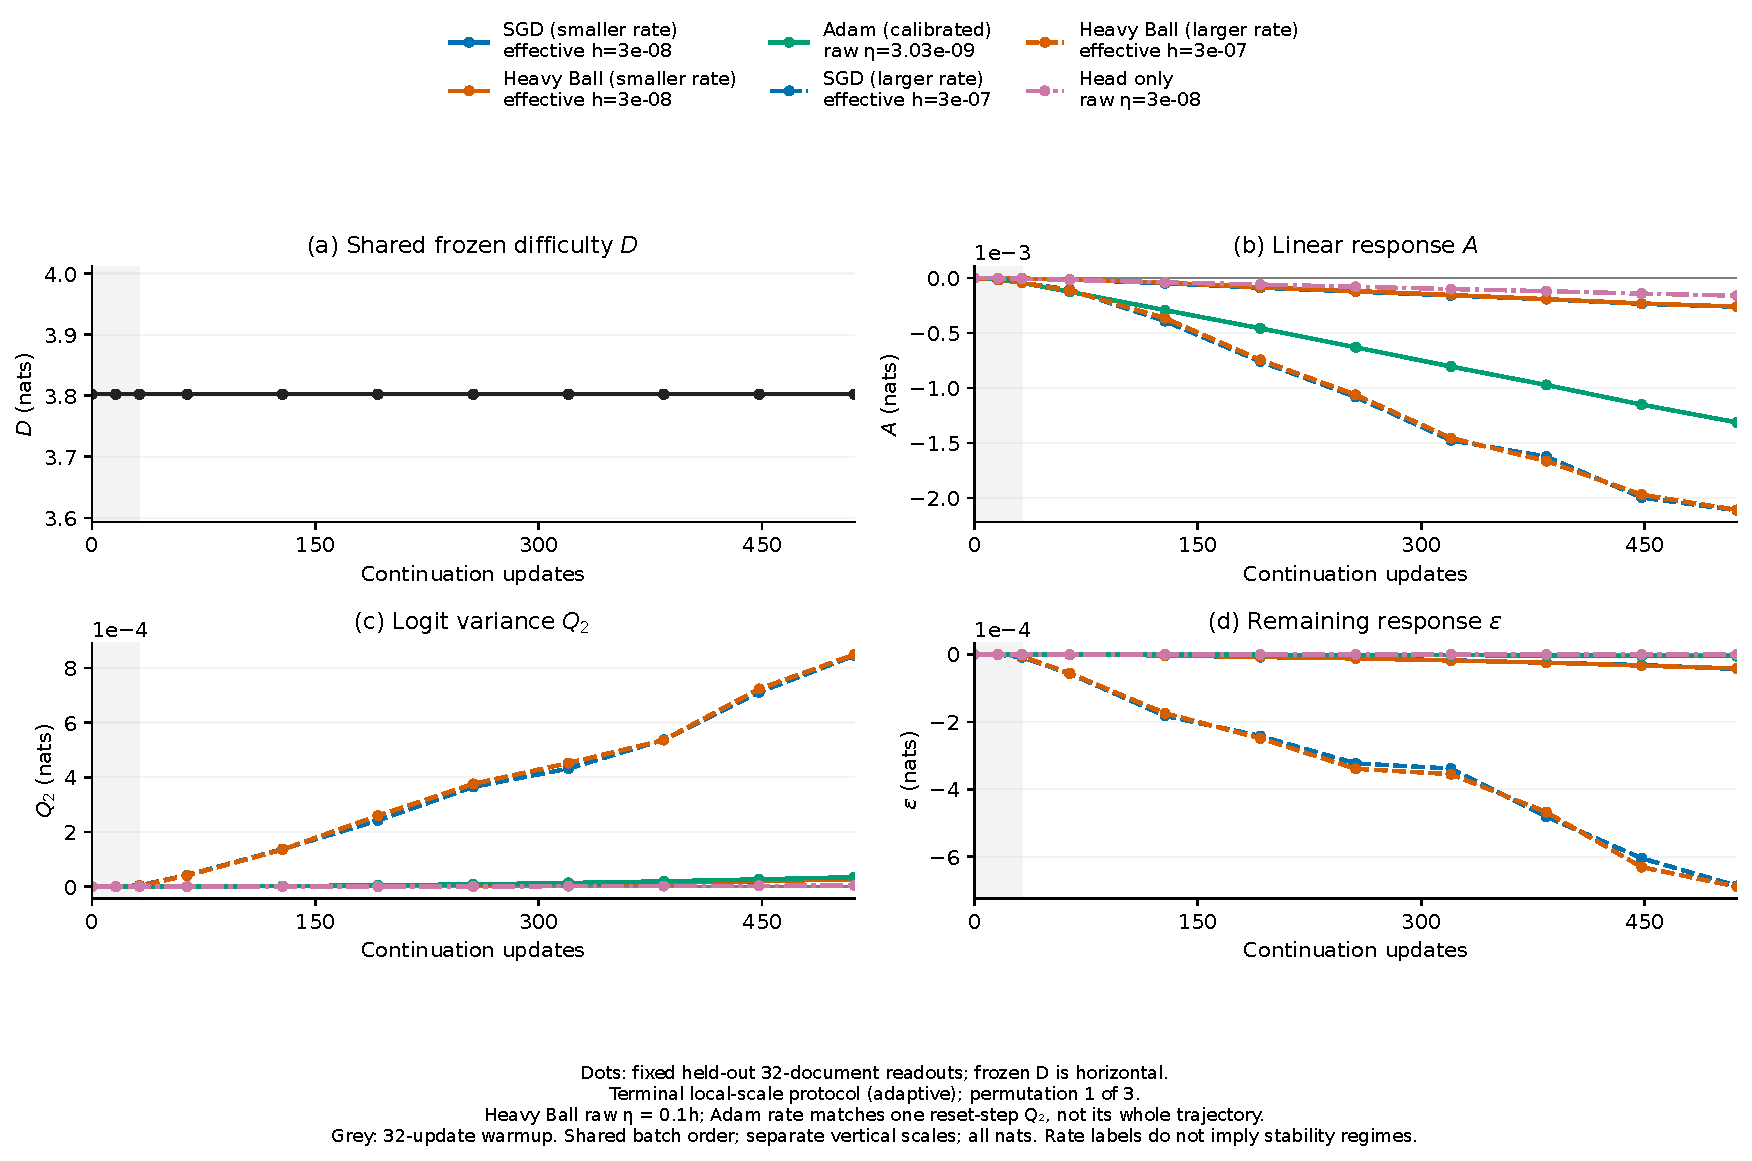
\includegraphics[width=\linewidth]{common-local-fixed.pdf}
\caption{The same decomposition on a fixed 32-document held-out probe.  Frozen $D$ is a horizontal line: its arriving-stream fluctuation in Fig.~\ref{fig:four-arrival} is batch composition, not a time-varying frozen predictor.  The other terms are scored at the prespecified readouts.  No curve is aligned by a fitted time warp.}
\label{fig:four-fixed}
\end{figure}

\paragraph{The output-head control identifies the network remainder.}
In the terminal protocol, full-model SGD's $\RMS(R)$ is $2.419\times10^{-5}$--$3.480\times10^{-5}$ nats, versus only $1.349\times10^{-7}$--$2.588\times10^{-7}$ for $\RMS(Q-Q_2)$.  HB has the same ordering.  Head-only $R$ is below $1.91\times10^{-14}$ nats in both smaller-rate protocols, as predicted by its affine logit map.  In the intermediate protocol, head-only closure passes at 2.24--2.42\%, while full SGD/HB fail at 33.83--44.66\% and 34.50--37.96\%.  The contrast separates network nonlinearity from the softmax approximation error using a function-preserving initial intervention.

\begin{table}[t]
\centering
\caption{Full-window response error $100\,\RMS(\varepsilon)/\RMS(L-D)$, in percent.  Ranges span all three permutations.  The registered gate is 10\%; rates label controlled interventions, not measured stability regimes.  The second and third protocols were adaptively registered after failures of the preceding smaller-rate pair.}
\label{tab:rate-validity}
\small
\setlength{\tabcolsep}{5pt}
\begin{tabular}{lrrr}
\toprule
Setting & Original & Intermediate & Terminal\\
\midrule
SGD, smaller rate &129.5--150.7 &33.83--44.66 &10.51--14.96\\
HB, smaller rate &200.3--222.7 &34.50--37.96 &10.56--15.21\\
Adam, calibrated &178.0--178.7 &19.97--20.39 &0.3387--0.3748\\
SGD, larger rate &862.3--1011.3 &47.68--48.97 &25.54--29.24\\
HB, larger rate &113.8--127.9 &47.82--50.89 &26.13--30.04\\
Head-only SGD &21.49--22.16 &2.24--2.42 &0.002410--0.002470\\
\midrule
Smaller effective rate & $3\!\times\!10^{-4}$ & $3\!\times\!10^{-6}$ & $3\!\times\!10^{-8}$\\
Larger effective rate & $1.2\!\times\!10^{-3}$ & $3\!\times\!10^{-5}$ & $3\!\times\!10^{-7}$\\
\bottomrule
\end{tabular}
\end{table}

The original large-rate settings also expose the probability-curvature boundary.  High SGD has mean $Q_2=11.33$--$13.10$ nats and a softmax-remainder RMS of 15.72--19.27 nats.  Calibrated Adam has a softmax-remainder RMS of 0.3140--0.3154 nats.  In these cases $Q_2$ is not an accurate substitute for the exact nonnegative $Q$.  This does not violate Eq.~\eqref{eq:exact}; it falsifies the useful quadratic approximation in that displacement regime.

\paragraph{Parameter alignment does not establish a constant token gap.}
At the terminal smaller rate, SGD/HB endpoint displacement cosine is 0.999706--0.999809 and relative distance 2.00--2.43\%.  At the intermediate smaller rate the cosine is 0.99107--0.99500; at the original smaller rate it is 0.73536--0.75361.  This supports better finite-time alignment as the registered rate decreases, at a fixed update count.  It is an endpoint displacement comparison, not a claim that every point on the trajectory coincides.

Even at the terminal smaller rate, paired arrival response closure fails at 22.18--28.30\%.  On the final probe, SGD/HB token gap has centered RMS $1.460\times10^{-4}$--$2.936\times10^{-4}$ nats and mean magnitude $1.569\times10^{-6}$--$3.141\times10^{-6}$.  The std/absolute-mean ratio is 46.49--163.48, far above 0.1.  The SGD/Adam ratio is 8.362--8.470.  Nearly aligned parameter motion and near-identical raw losses therefore coexist with a heterogeneous small paired gap.  These continuations do not establish the stronger nonzero constant-offset RGI property.

\begin{figure}[t]
\centering
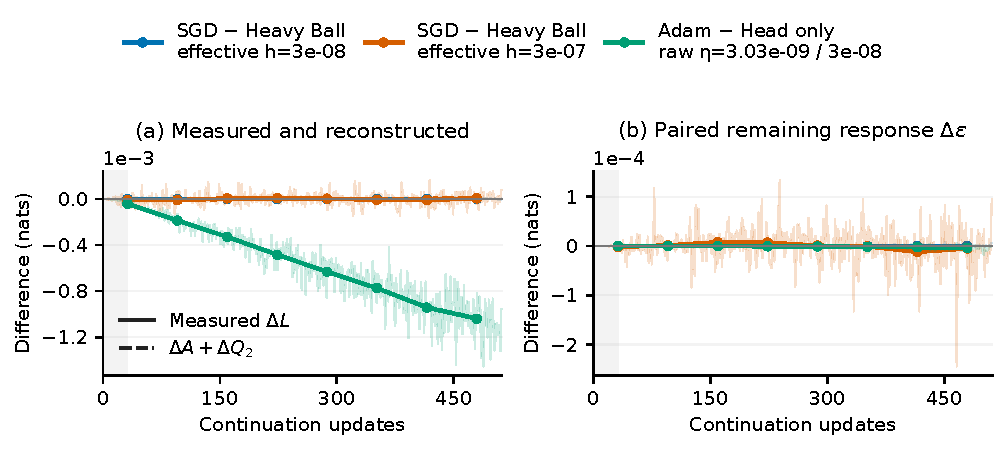
\includegraphics[width=\linewidth]{common-local-paired.pdf}
\caption{Paired response and measured remaining discrepancy after the exactly shared $D$ cancels.  Raw values and prespecified block means are retained.  This scale reveals sample-conditioned differences that a raw-loss plot can hide.}
\label{fig:paired-response}
\end{figure}

\section{Same-stream momentum alignment and its limits}
\label{sec:alignment-theory}

The common-checkpoint design admits an exact comparison that does not require slowly varying stochastic batch gradients.  Let \(s_{t+1}=s_t-h_tg_t(s_t)\) be SGD and \(m_{t+1}=m_t-h_tv_t\) normalized Heavy Ball on the same prescribed sequence of batch objectives, with
\(v_t=\beta v_{t-1}+(1-\beta)g_t(m_t)\), \(v_{-1}=0\), and \(s_0=m_0\).
Writing \(e_t=m_t-s_t\) and \(k=\beta/(1-\beta)\), summation by parts gives the exact finite-time identity
\begin{align}
 e_T={}&-\sum_{t<T}h_t\{g_t(m_t)-g_t(s_t)\} \nonumber\\
 &+k\left[h_{T-1}v_{T-1}-\sum_{t<T-1}(h_{t+1}-h_t)v_t\right].
 \label{eq:memory-defect}
\end{align}
The first term is gradient feedback from the divergent parameters; the second is an explicit memory and warmup contribution.  In particular, reset momentum has a genuine startup transient even at matched dc gain.  We preserve it in the measured curves.

If every batch gradient is \(\Lambda\)-Lipschitz on a common region containing both paths and \(\|g_t(m_t)\|\le G\), a nondecreasing warmup to \(h_{\max}\) gives
\begin{equation}
 \|e_T\|\le 2\frac{\beta}{1-\beta}h_{\max}G
   \exp\!\left(\Lambda\sum_{t<T}h_t\right).
 \label{eq:momentum-bound}
\end{equation}
Indeed \(\|v_t\|\le G\), the bracket in Eq.~\eqref{eq:memory-defect} has norm at most \(2h_{\max}G\), and discrete Gronwall yields the result.  With a constant rate the leading two can be replaced by one.  This establishes an alignment limit as \(h_{\max}\to0\) at fixed integrated progress under uniform regularity.  The bound can be loose, and our measurements do not estimate \(\Lambda\) or \(G\); a same-update-count rate contrast is not a numerical proof of the fixed-progress asymptotic statement.

On a fixed probe, \(|\Delta A|\le\|g_B(\theta_0)\|\|e_T\|\).
For the frozen categorical covariance seminorm \(\|\cdot\|_{C_B}\),
\begin{equation}
 |\Delta Q_2|\le\tfrac12\|\Delta z_a-\Delta z_b\|_{C_B}
    (\|\Delta z_a\|_{C_B}+\|\Delta z_b\|_{C_B}).
 \label{eq:variance-bound}
\end{equation}
Actual function alignment consequently constrains the first two response differences; \(\Delta\varepsilon\) and centered token gaps must still be checked.  These equations do not cover Adam or imply a sample-independent nonzero offset.

\section{Limitations and conclusion}

The measurements support a specific local story.  The large fast fluctuation is the difficulty of the arriving targets under a fixed predictor.  Once that term is removed, the realized finite response is well described on average by the batch's frozen gradient acting on the observed displacement plus the positive curvature cost of moving probabilities.  Linear work generates the loss decrease; softmax curvature offsets part of it.  The optimizer changes both terms, and the network representation residual becomes visible when spans are long or when two optimizer responses are subtracted.

The result does not establish the stronger claim that natural Transformer training universally preserves a constant token-wise optimizer offset.  The scalar probe fails to describe batch-specific response, the optimizer-difference closure fails its registered 10\% RMS gate, and the known-teacher population gap varies strongly across prefixes.  The original RGI phenomenon and the local decomposition can therefore coexist: shared difficulty can produce very high loss correlation while the smaller paired gap remains structured.

The study has four scope limits.  It uses a Pythia-70M local continuation rather than the original paper's 124M and 0.7B from-scratch runs; the three permutations share one data pool; the data's overlap with Pythia pretraining is unknown; and the response diagnostics use observed finite displacements.  The independent checks audit saved arithmetic and fixtures but do not rerun the full gradients or optimizer trajectories.

The practical theoretical target is now concrete.  A future test of strong RGI should measure candidate support mass and within-support shape, record batch-specific gradient response, and prospectively evaluate an unseen window.  It should not infer a universal mechanism from a quadratic sufficient example or from the exact identity \(W+Q\).  Our current evidence identifies the dominant terms in the finite Pythia-70M continuation and an explicit obstruction to extending them to a universal Transformer law.


\bibliographystyle{plainnat}
\bibliography{references}

\appendix
\section{Reproducibility details}

\paragraph{Data and model hashes.}
The FineWeb source is \texttt{HuggingFaceFW/fineweb}, configuration \texttt{sample-10BT}, revision prefix \texttt{9bb295dd}, shard \texttt{sample/10BT/001\_00000.parquet}.  The pool selection starts after source row 65,536 and uses selection seed 610000 and split seed 610001.  The verified tokenizer commit begins \texttt{a39f36b1}.  The public release includes a bounded selection-contract extract and artifact hashes in its evidence directory; raw document/token manifests are not included.

\paragraph{Evaluation units.}
Natural batches contain 8 documents and 223 scored next-token targets per document (query positions 32 through 254).  Difficulty and response statistics are computed from document-level means; token positions within a document are not treated as independent documents.  The known-teacher continuation uses 33 natural seed tokens followed by 63 sampled tokens and evaluates 63 targets per generated document.

\paragraph{Verification scope.}
The extension, logit-work, and arrival verifiers report 23,220, 4,159, and 341 passed checks, respectively, with maximum reported arithmetic errors of \(8.88\times10^{-15}\), \(3.17\times10^{-14}\), and \(3.56\times10^{-15}\).  These checks cover trace parity, hashes, document aggregation, exact identities, and saved full-vocabulary fixtures.  They do not independently recompute the full network gradients, the optimizer trajectory, or every saved logit from raw checkpoints.  The arrival and work analyses are therefore numerical audits of recorded runs, not independent training replications.

\paragraph{Additional diagnostics.}
The registered 64-step block analysis uses signed covariance shares; these shares are attribution coefficients and may exceed one or be negative because terms cancel.  High-pass SGD failures and the optimizer-difference failure are retained in the main text rather than averaged away.  The three permutations reuse one data pool and are not independent datasets.

\paragraph{Code and artifacts.}
The arXiv source package contains the main manuscript, the MetaCircle style assets, the numerical-theory figure, and the compiled bibliography.  The public release additionally contains machine-readable aggregate analyses, chart values, and provenance hashes. It excludes raw checkpoints, full logits, producer traces, and training-data text; it is not a complete training reproduction package.

\section{Historical distinct-start diagnostics}
The earlier study used optimizer-specific continuation starts and a common step-32,000 scoring reference.  It is retained as historical evidence and does not replace the common late-checkpoint experiment.  Its main scales were \(\operatorname{std}(D)=0.1843\)--\(0.1937\), mean \(A=-0.004011\)--\(-0.003552\) (SGD) and \(-0.003290\)--\(-0.003272\) (Adam), mean \(Q_2=0.001744\)--\(0.001992\) and \(0.000622\)--\(0.000634\), and \(\RMS(\varepsilon)=0.000191\)--\(0.000286\) and \(0.0000754\)--\(0.0000838\) nats.  These small-remainder values are not transferred to the later common checkpoint or newly calibrated rates.
\section{Known-teacher continuation}

The natural experiment has no observed conditional distribution, so its reference decomposition cannot decide whether the target residual is label noise or a systematic model mismatch.  The known-teacher experiment removes that ambiguity.  For the fixed teacher \(q\), the population objective is exactly \(H(q)+\KL(q\Vert p)\), while hard targets additionally expose the sampled terms \(S\) and \(C\) in Eq.~\eqref{eq:teacher}.

The teacher entropy averages 4.1798397 nats, the sampled teacher surprisal averages 4.1723279 nats, and the initial teacher KL of the student probe is 0.2593348 nats.  After 128 updates, teacher KL ranges are 0.229442--0.229879 for hard SGD, 0.241563--0.241657 for hard Adam, 0.228137--0.228251 for soft SGD, and 0.229840--0.229902 for soft Adam.  The population \(A+Q_2\) closure error is at most 2.795\% across the tested horizons, objectives, and permutations.

The term means show why a KL-only explanation is incomplete.  In hard-teacher SGD at 128 updates, the mean linear work is about \(-0.057\) nats, curvature is about \(+0.027\), and the net risk change is about \(-0.030\).  In hard-teacher Adam the corresponding values are about \(-0.022\), \(+0.004\), and \(-0.018\).  Soft targets change both magnitudes.  The cancellation is a finite-displacement observation and does not establish that two optimizers share a common first-order coefficient.

The same control also tests strong RGI.  After exact teacher-population integration, the cross-prefix standard deviation of the hard optimizer gap divided by its absolute mean is 3.59--3.69; the soft value is 10.69--11.89.  Both are far above a strict 0.1 constant-offset threshold.  Removing sampled-label noise therefore does not recover a uniform optimizer shift across prefixes.

\section{A sufficient support-gate construction}

For completeness, consider a prefix \(x\) with a known support \(S_x\), a normalized shape \(p_x\) on that support, and a reject token.  Let
\begin{equation}
 q_h(y\mid x)=\alpha(h)p_x(y)\quad (y\in S_x),\qquad
 q_h(\mathrm{reject}\mid x)=1-\alpha(h),
 \label{eq:support-gate}
\end{equation}
where \(\alpha(h)=\operatorname{sigmoid}(h)\).  For every target in the support,
\begin{equation}
 \ell_h(x,y)=-\log p_x(y)-\log\alpha(h),
 \qquad \partial_h\ell_h=\alpha(h)-1.
 \label{eq:gate-loss}
\end{equation}
Thus all target losses share the same algorithm-dependent offset, even though the common target surprise varies with \(p_x(y)\).  A dog/cat numerical check gives a gap 0.5901707965 with standard deviation \(1.05\times10^{-16}\) across five prefixes and both targets.

This is a sufficient support-gate mechanism, not evidence about natural LLMs.  It relies on a common normalized shape inside a prefix-dependent support and on a shared scalar mass gate.  Full-support language distributions have no reject mass with which to implement this exact construction.  Measuring whether natural models have an approximate candidate support and a common mass gate is a separate experiment.

\end{document}
